% Inbuilt themes in beamer
\documentclass{beamer}


%Defining some colours
\definecolor{darkred}{rgb}{0.8,0,0}

% Theme choice: there a number of preset themes to choose from
% Play around with them, Cambridge is nice for first pres
%\usetheme{Szeged}
\usetheme{CambridgeUS} %setting the main theme
%\usecolortheme{beaver} % setting colour theme
\usefonttheme{professionalfonts} %font theme
\useinnertheme[shadow=true]{rounded}
%\useoutertheme{} %outer theme

%\setbeamertemplate{footline} %Remove footer line in all slides
\setbeamertemplate{navigation symbols}{} %removes navigation symbols
\setbeamertemplate{footline}[page number] %removes footer line, keeps pg#
\setbeamertemplate{caption}{\insertcaption} 

%Setting colours for boxes and captions
\setbeamercolor{block title}{bg=darkred, fg=white}
\setbeamercolor{block body}{bg=darkred!10}

% For the Flowchart
\usepackage{tikz}
\usetikzlibrary{shapes.geometric, arrows}
\tikzstyle{startstop} = [rectangle, rounded corners, minimum width=3cm, minimum height=1cm,text centered, draw=black, fill=red!30]
\tikzstyle{process} = [rectangle, minimum width=3cm, minimum height=1cm, text centered, draw=black, fill=orange!30]
\tikzstyle{decision} = [diamond, minimum width=3cm, minimum height=1cm, text centered, draw=black, fill=green!30]
\tikzstyle{arrow} = [thick,->,>=stealth]


% Title page details: 
\title[BEAP Dec 2022]{Cells at War 2021 Survey Data } 
\author{Alexander Turco}
\date{March 10, 2022}
%\logo{
\includegraphics[height=1cm, width=1cm]{logo.png}}

% Bibliography stuff
\usepackage[natbib=true, sorting=nyt, style=authoryear-comp]{biblatex}
\addbibresource{ABC1.bib}

%Extra packages
\usepackage{makecell}

%For itemize
\setbeamertemplate{itemize item}[triangle]



\begin{document}
	
	% For my introduction slides, there will be the slide with my title and name as well as an outline slide with the brief overview of what I will discuss.
	% Title page frame - SLIDE 1%%%%%%%%%%%%%%%%%%%%%%%%%%%%%%%%%%%%%%%%%%%%%%%%%%%%%%%%%%%%%%%%%%%%%%%%%%%%%%%%%%%%%%%%%%%%%%%%%%%%%%%%%%%%%%%%%%%%%%%%%%%%%%%%%%%%
	\section{Figures}
	\begin{frame}
		\titlepage 
	\end{frame}
	
	% Remove logo from the next slides
	%\logo{}
	
	% Outline frame - SLIDE 2
	\begin{frame}{On average, how much time do you spend playing video games each week?}
		
		\begin{center}
			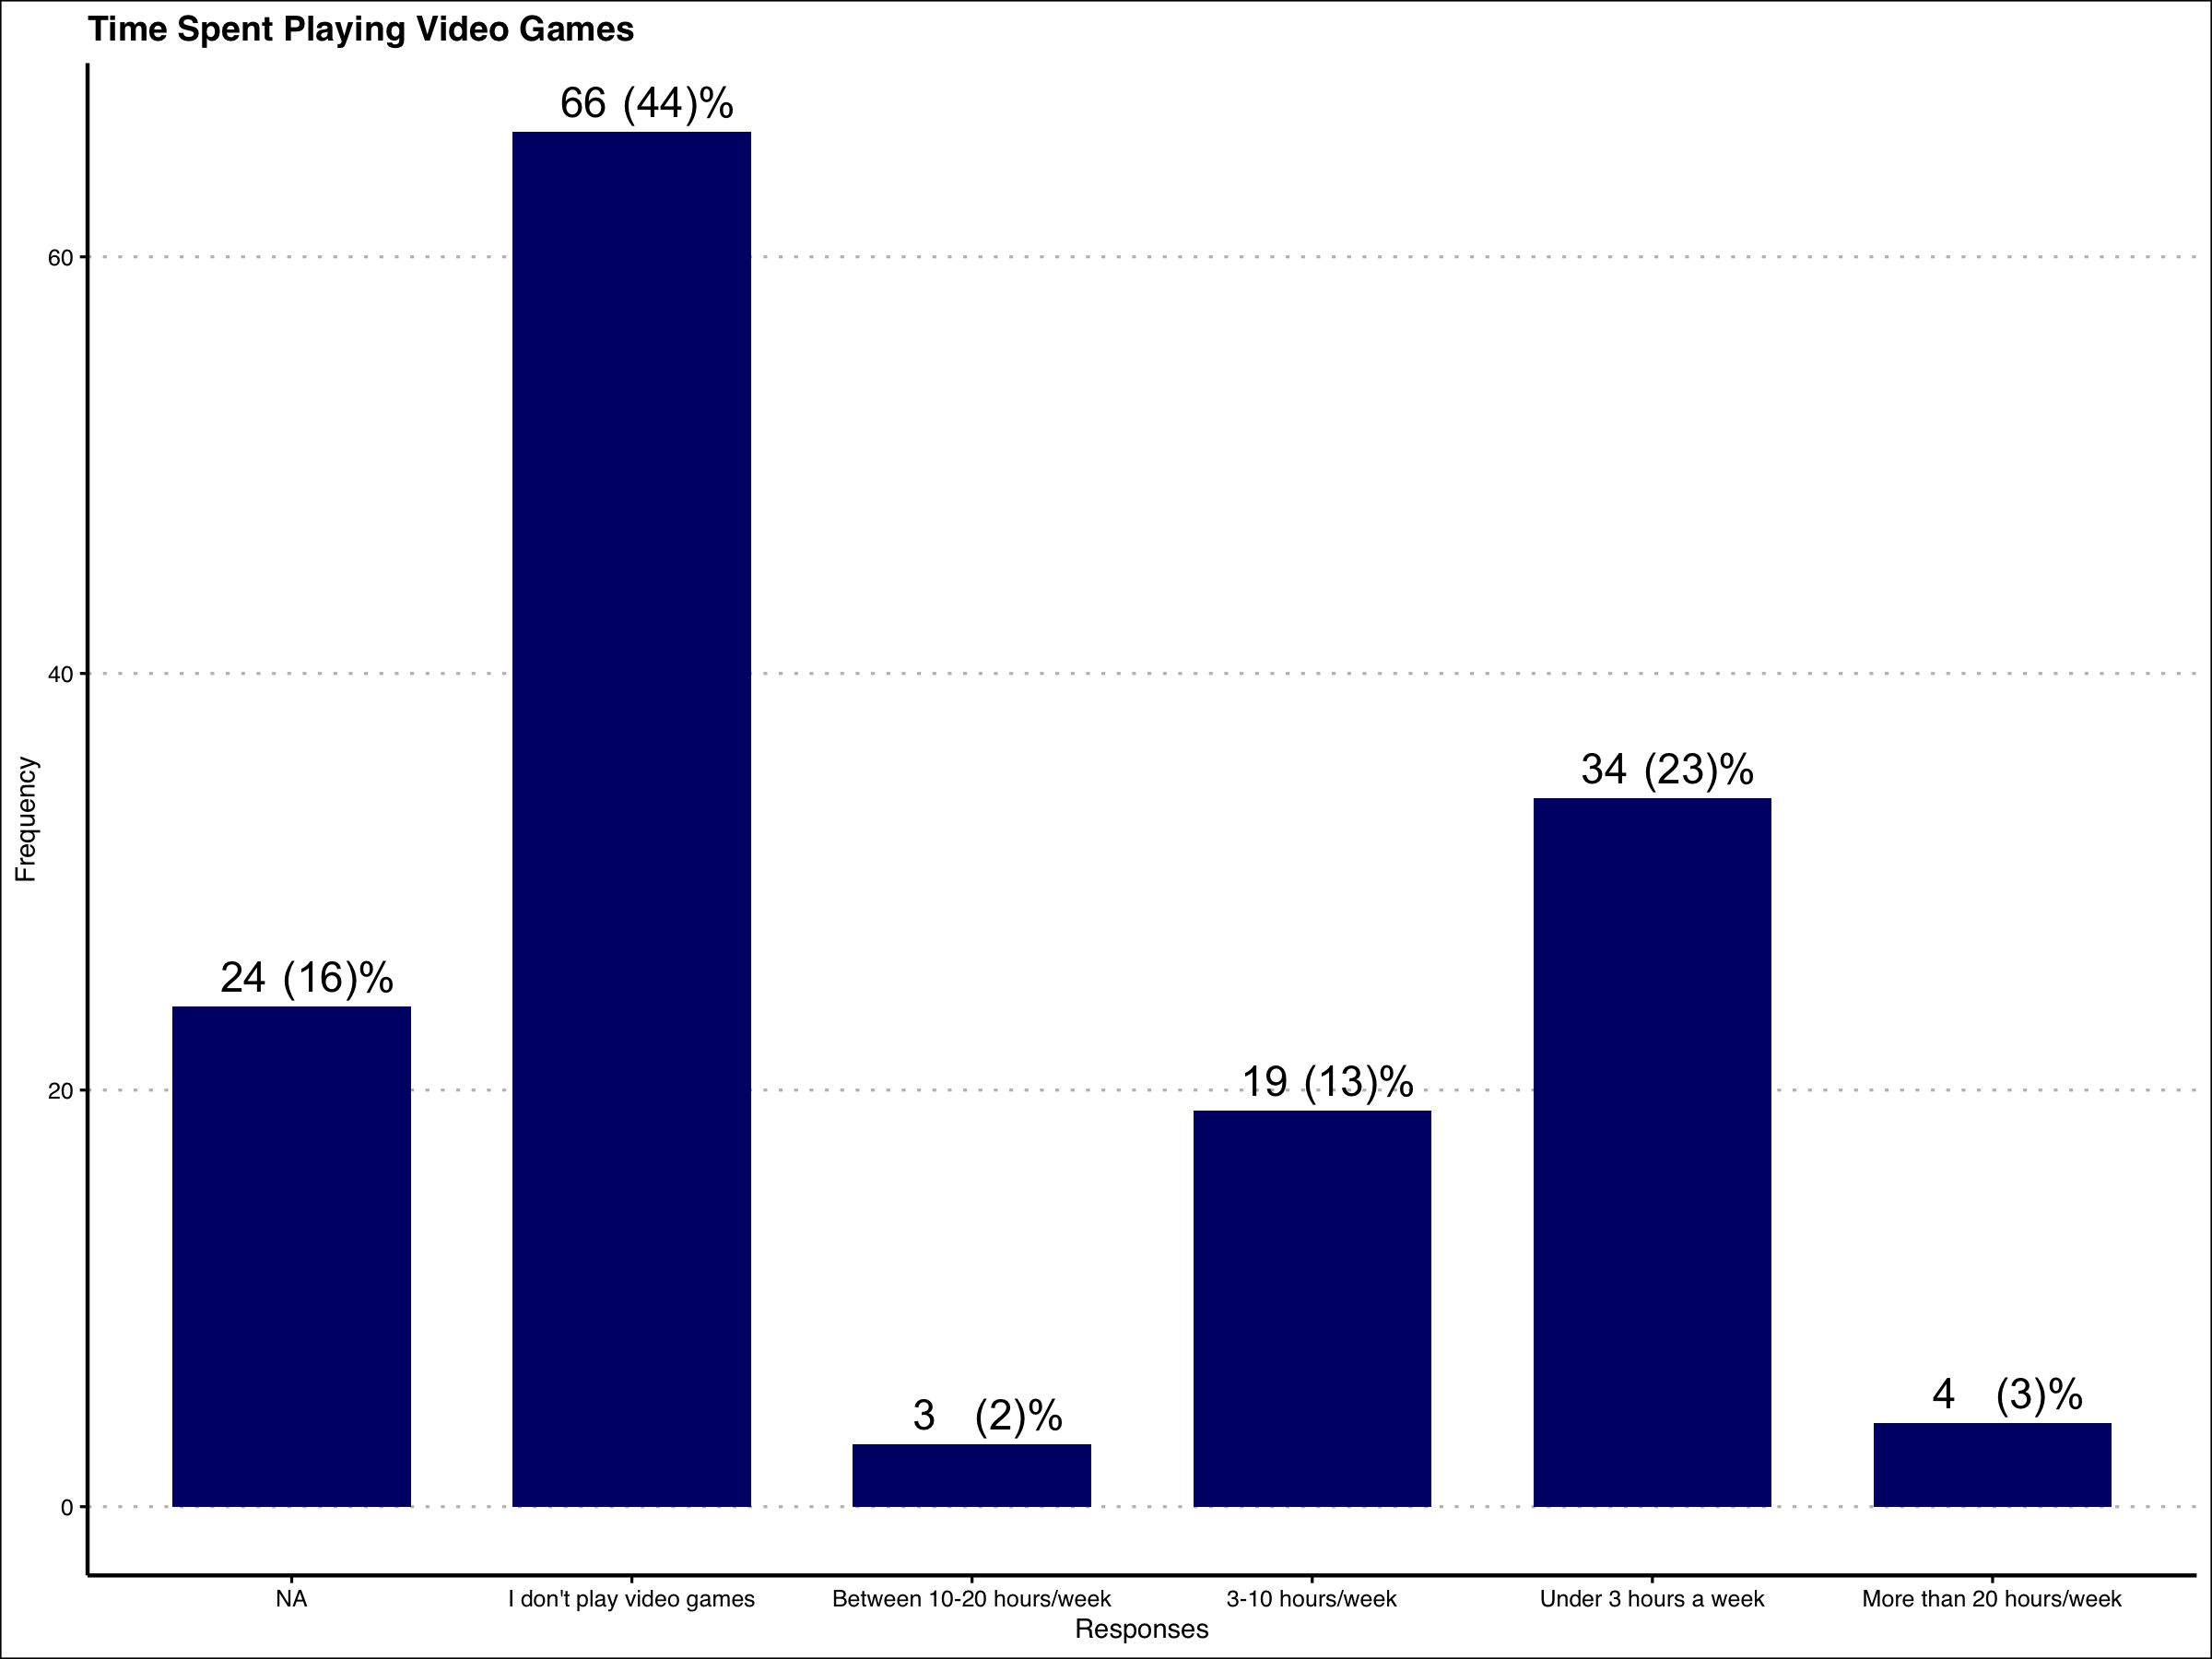
\includegraphics[width=10cm, height=7cm]{figures/time_spent_playing_videogames.jpg}
		\end{center}
	
	\end{frame}

	\begin{frame}{What types of courses have you taken at McMaster this current school year?}
		
		\begin{center}
			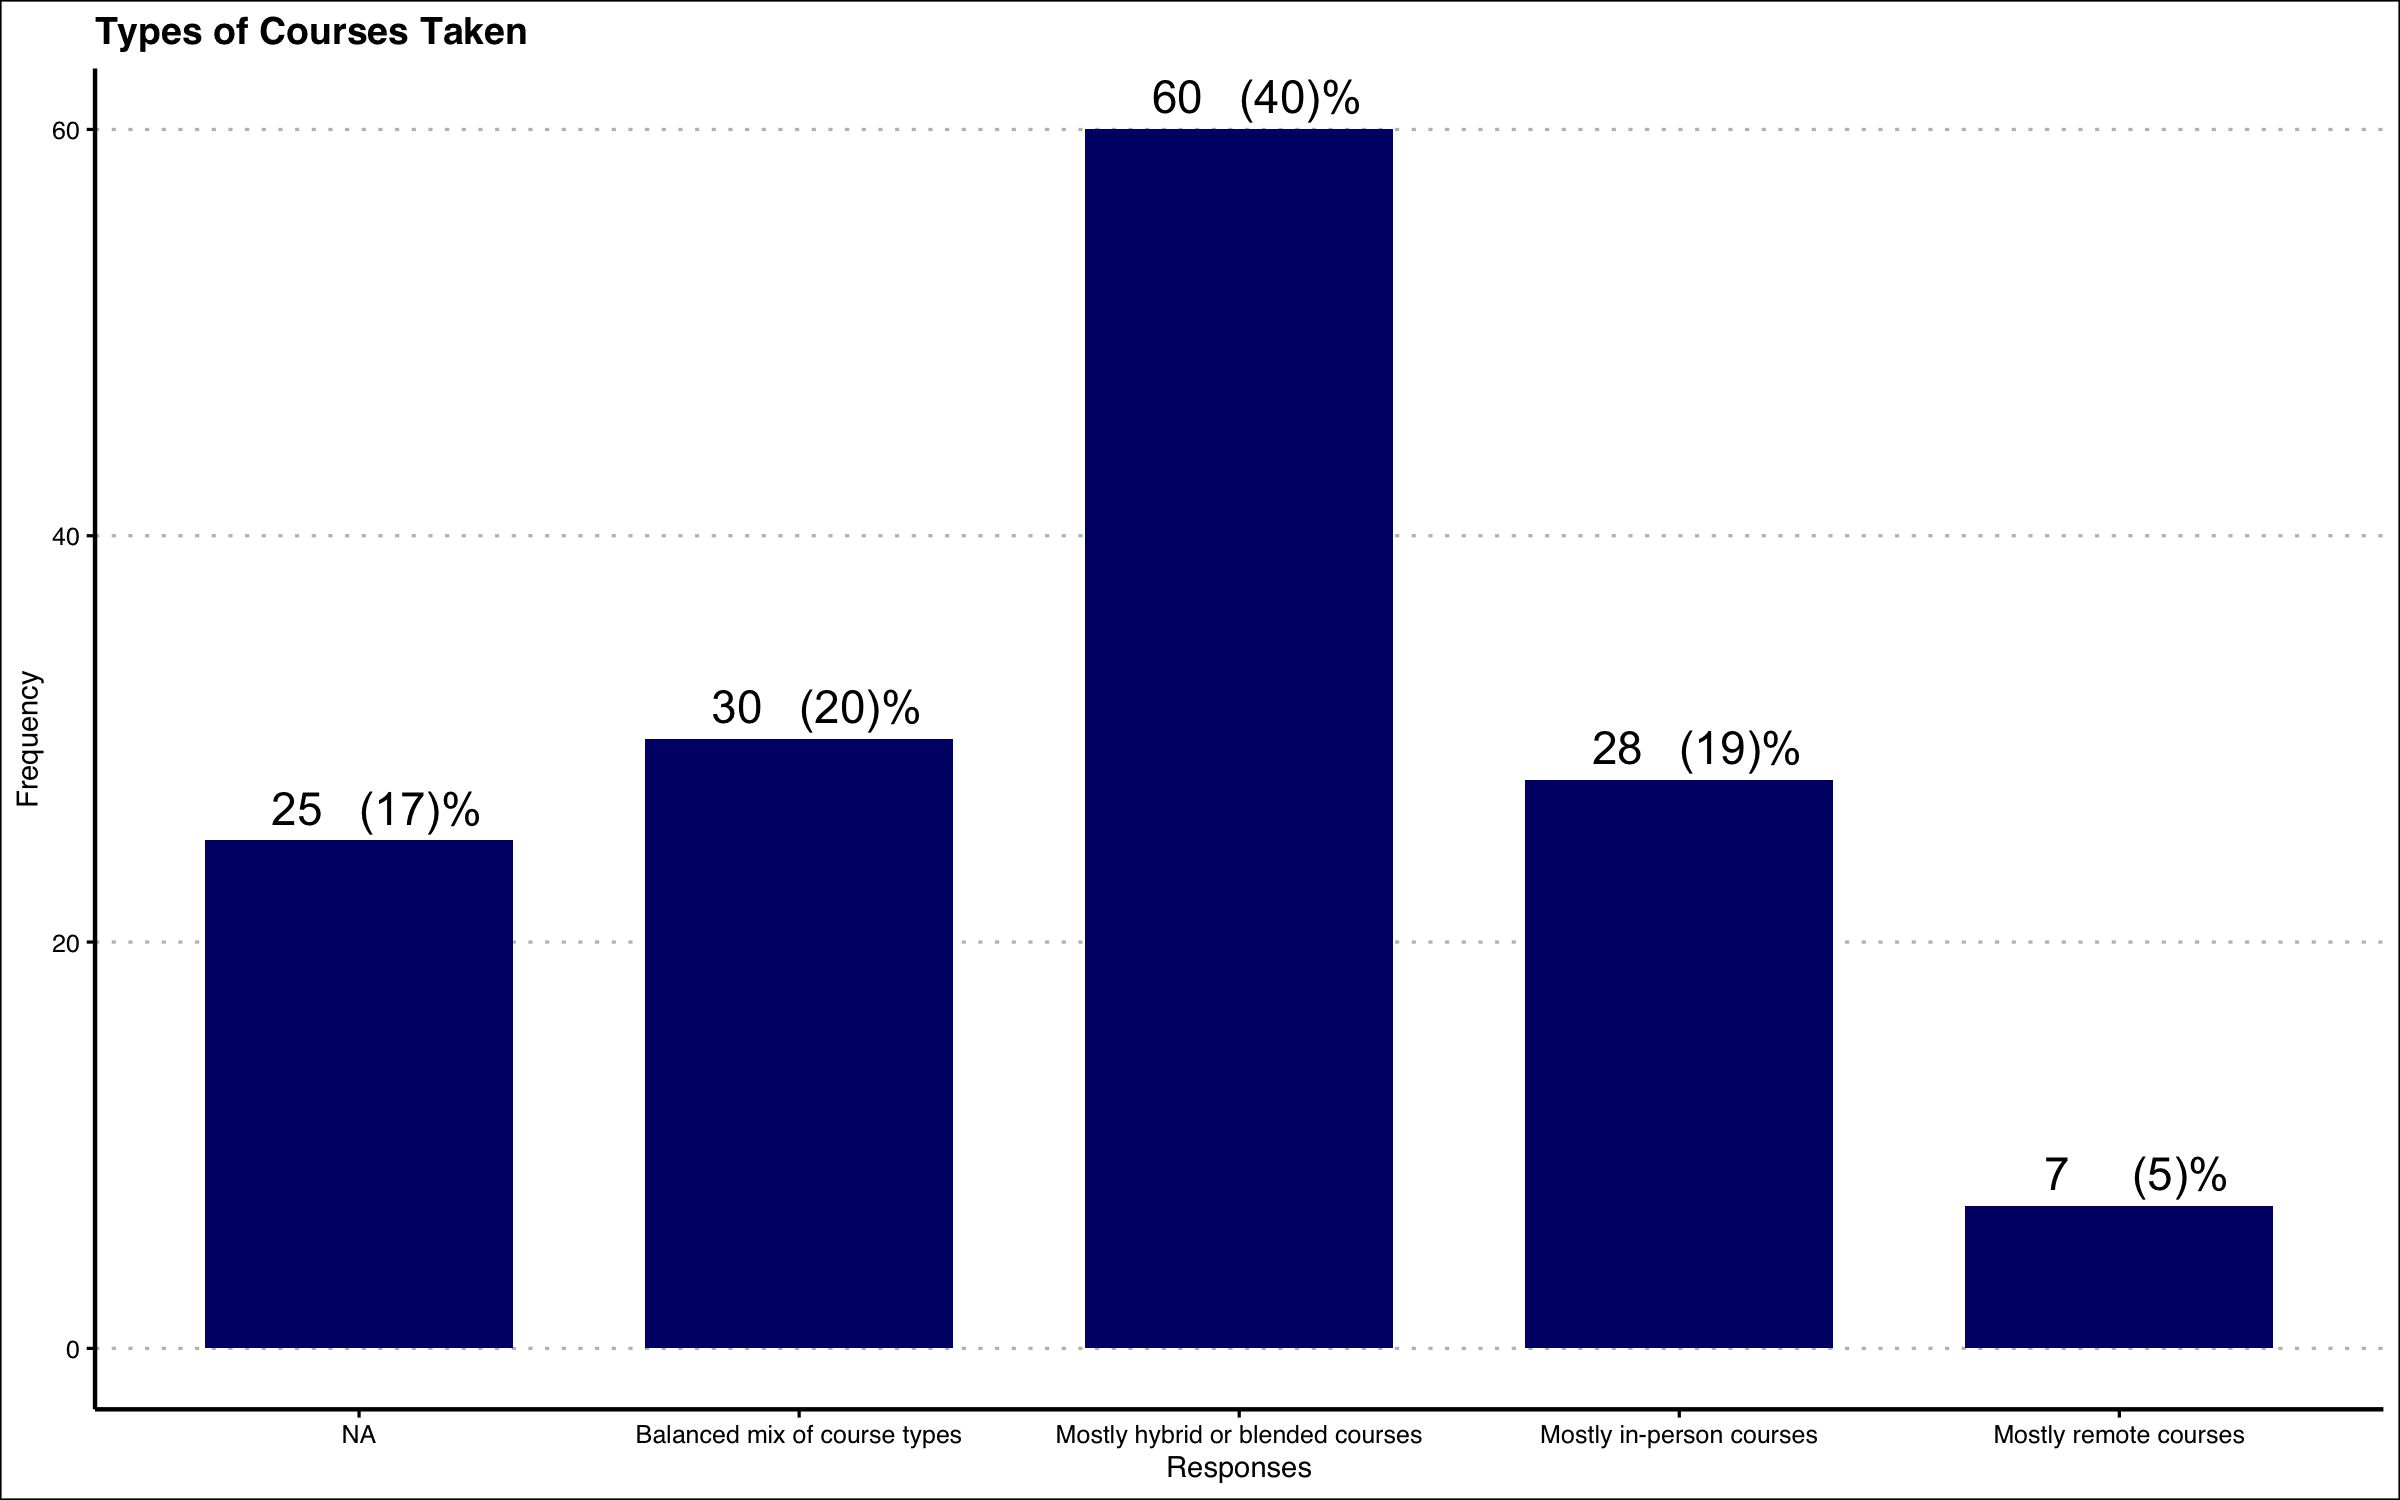
\includegraphics[width=10cm, height=7cm]{figures/types_of_courses_taken.jpg}
		\end{center}
		
	\end{frame}

	\begin{frame}{During the current school year, how often would you say you have done the following?}
		
		\begin{center}
			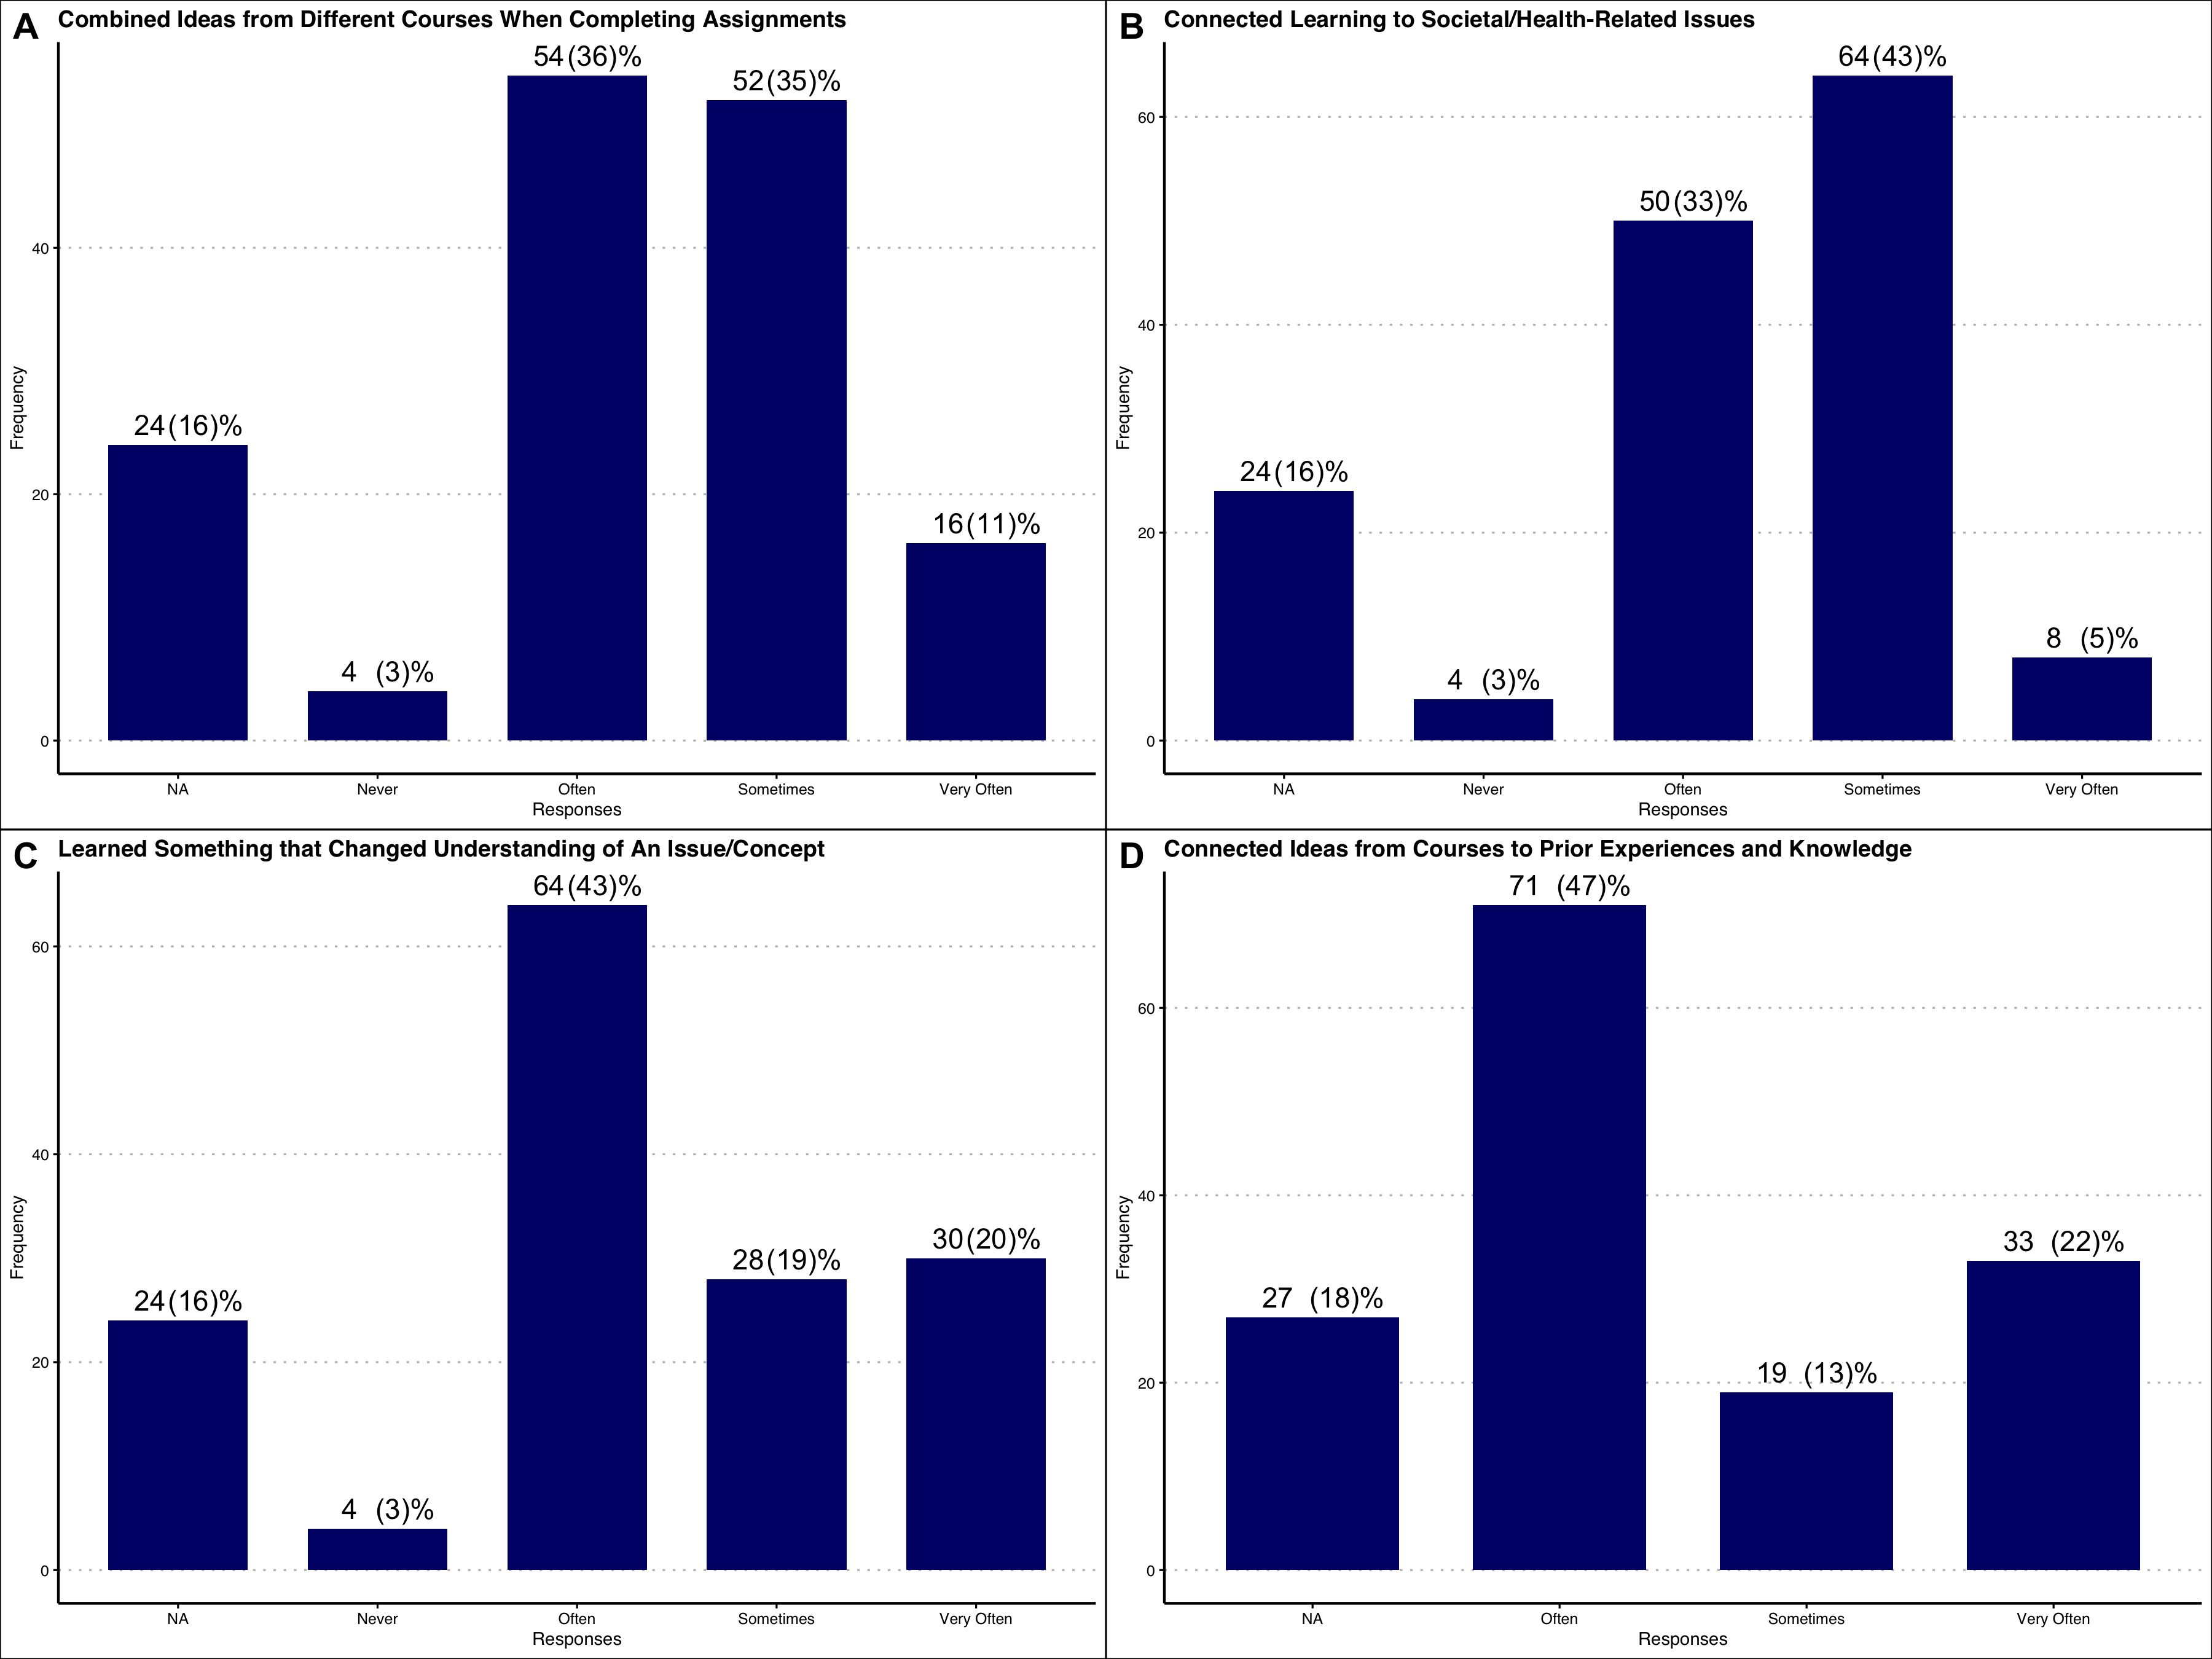
\includegraphics[width=10cm, height=7cm]{figures/how_often_haveyou_done_thefollowing.jpg}
		\end{center}
		
	\end{frame}

	\begin{frame}{During the current school year, how much would you say your coursework has emphasized the following? }
		
		\begin{center}
			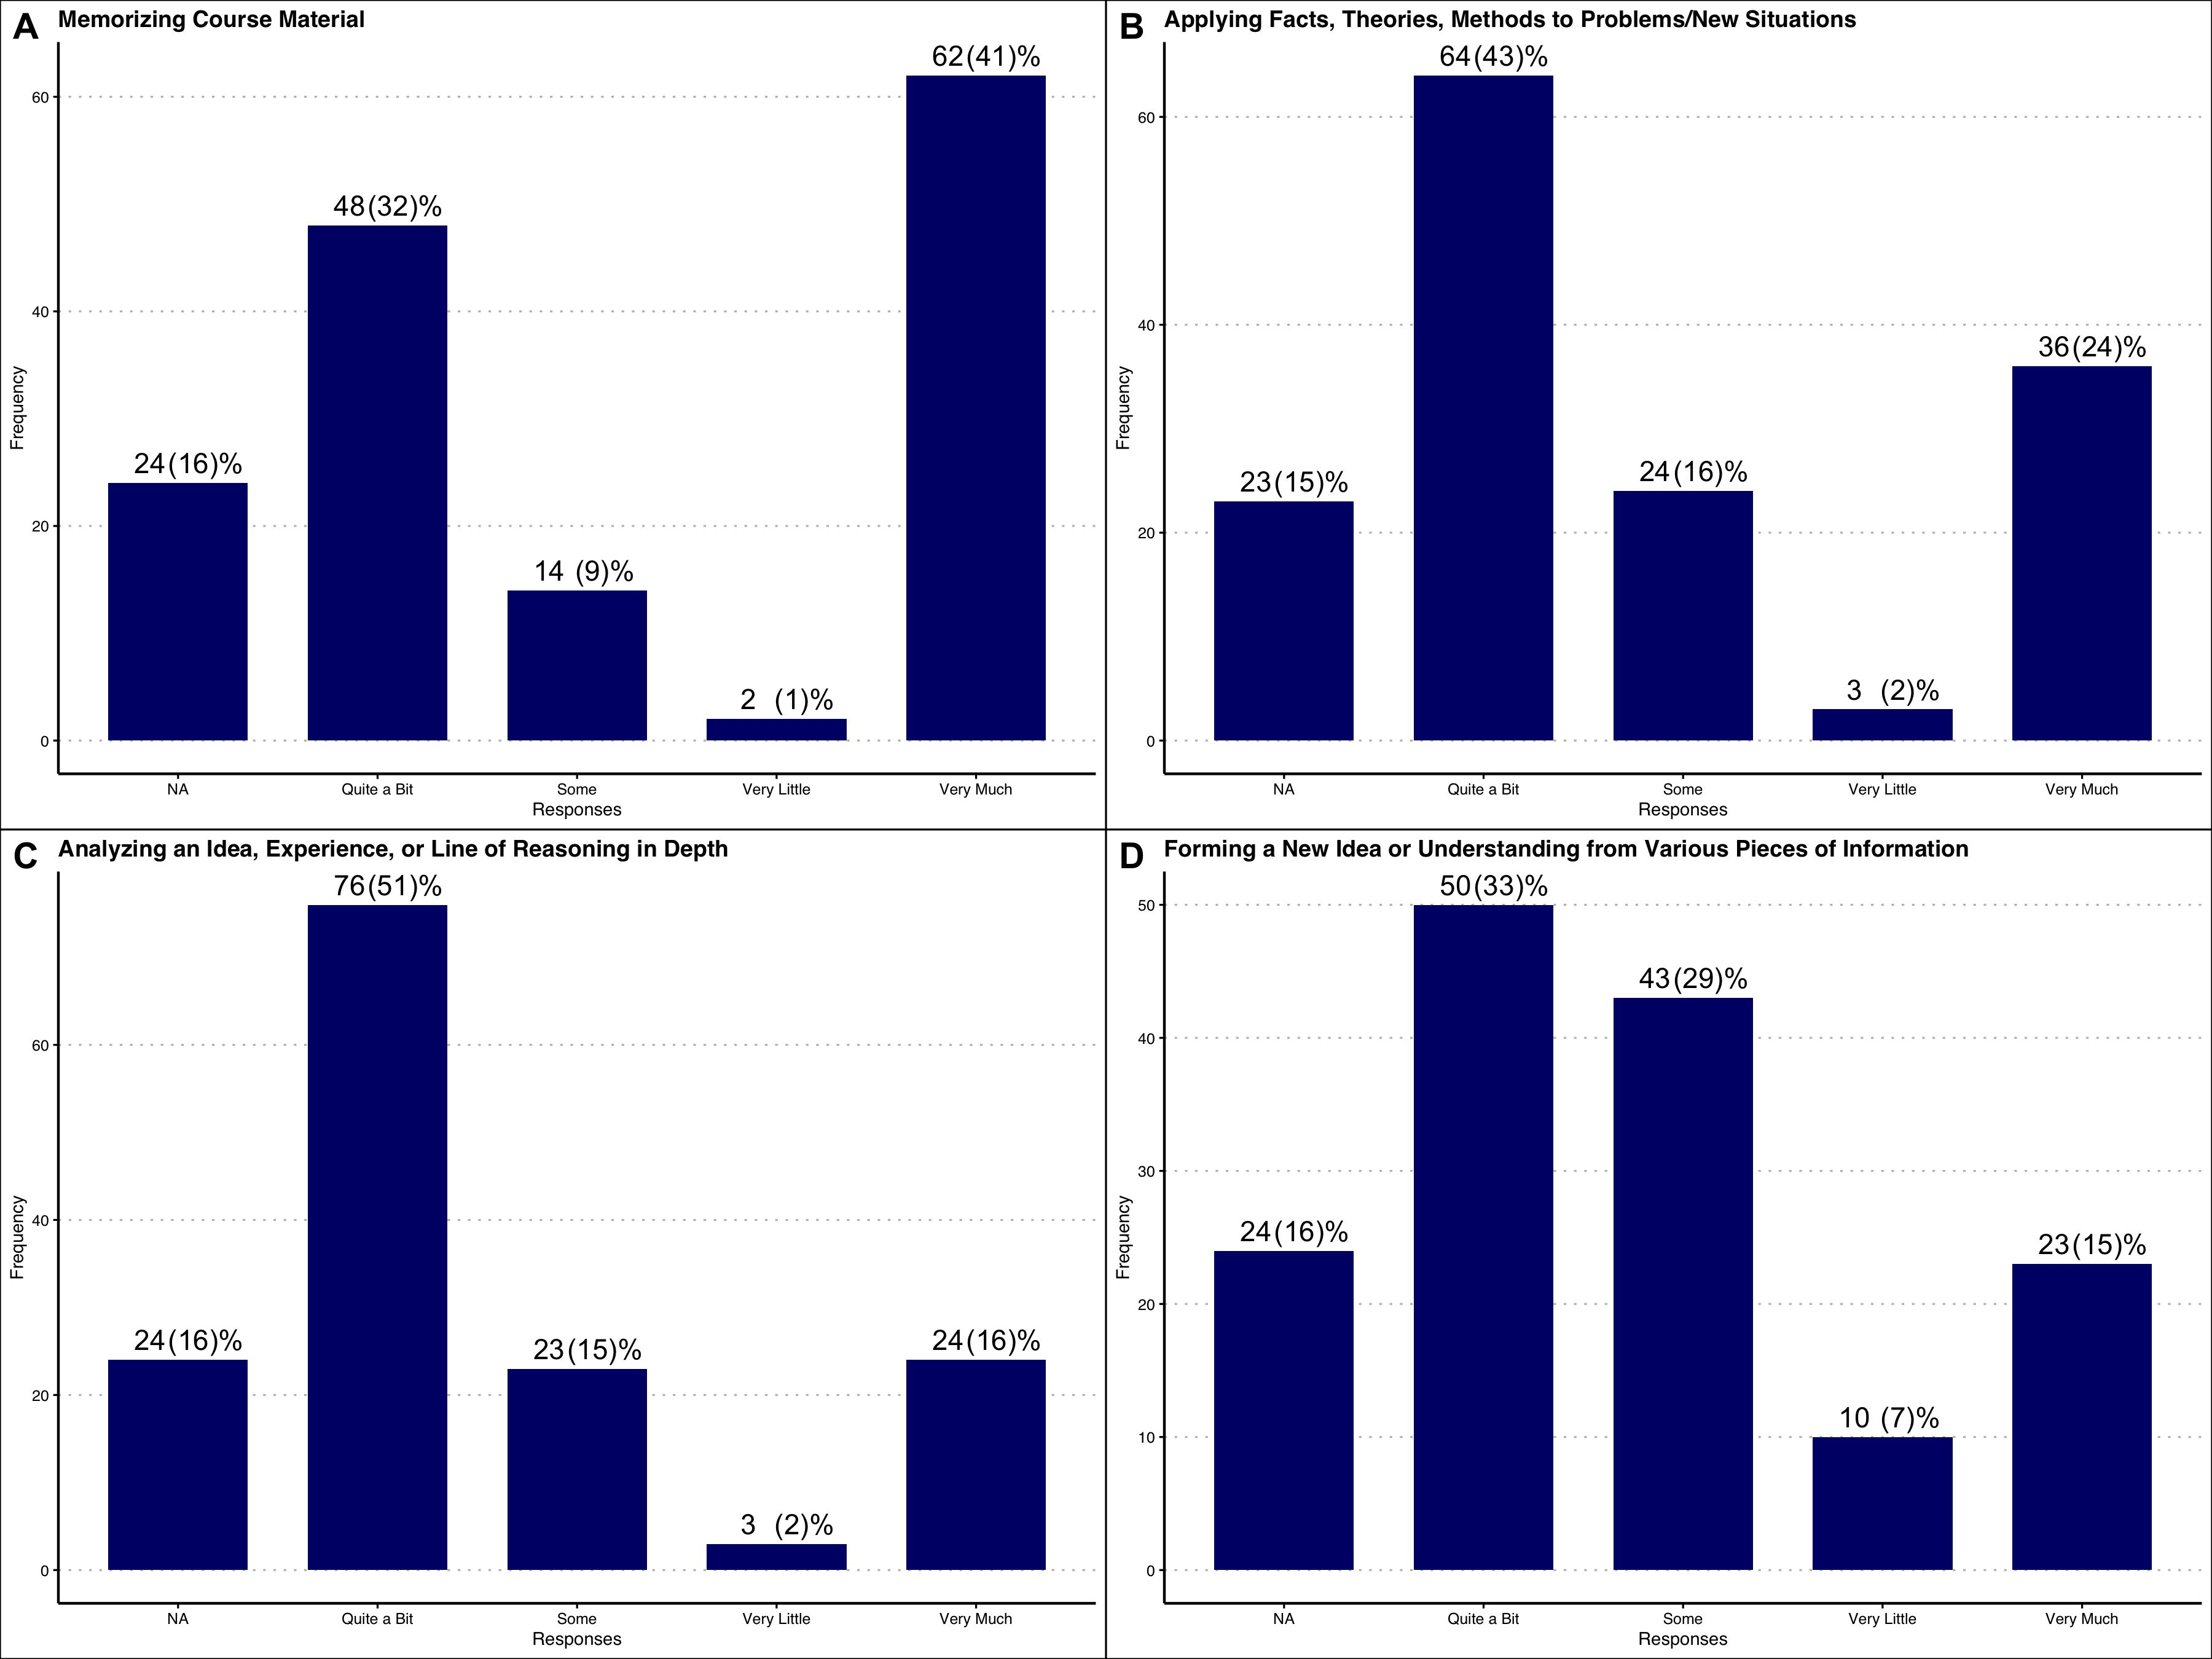
\includegraphics[width=10cm, height=7cm]{figures/howmuch_coursework_emphasized_thefollowing.jpg}
		\end{center}
		
	\end{frame}

	\begin{frame}{If game-based learning approaches were incorporated into one of your science courses, how do you think that this mode of learning can help with the following? }
		
		\begin{center}
			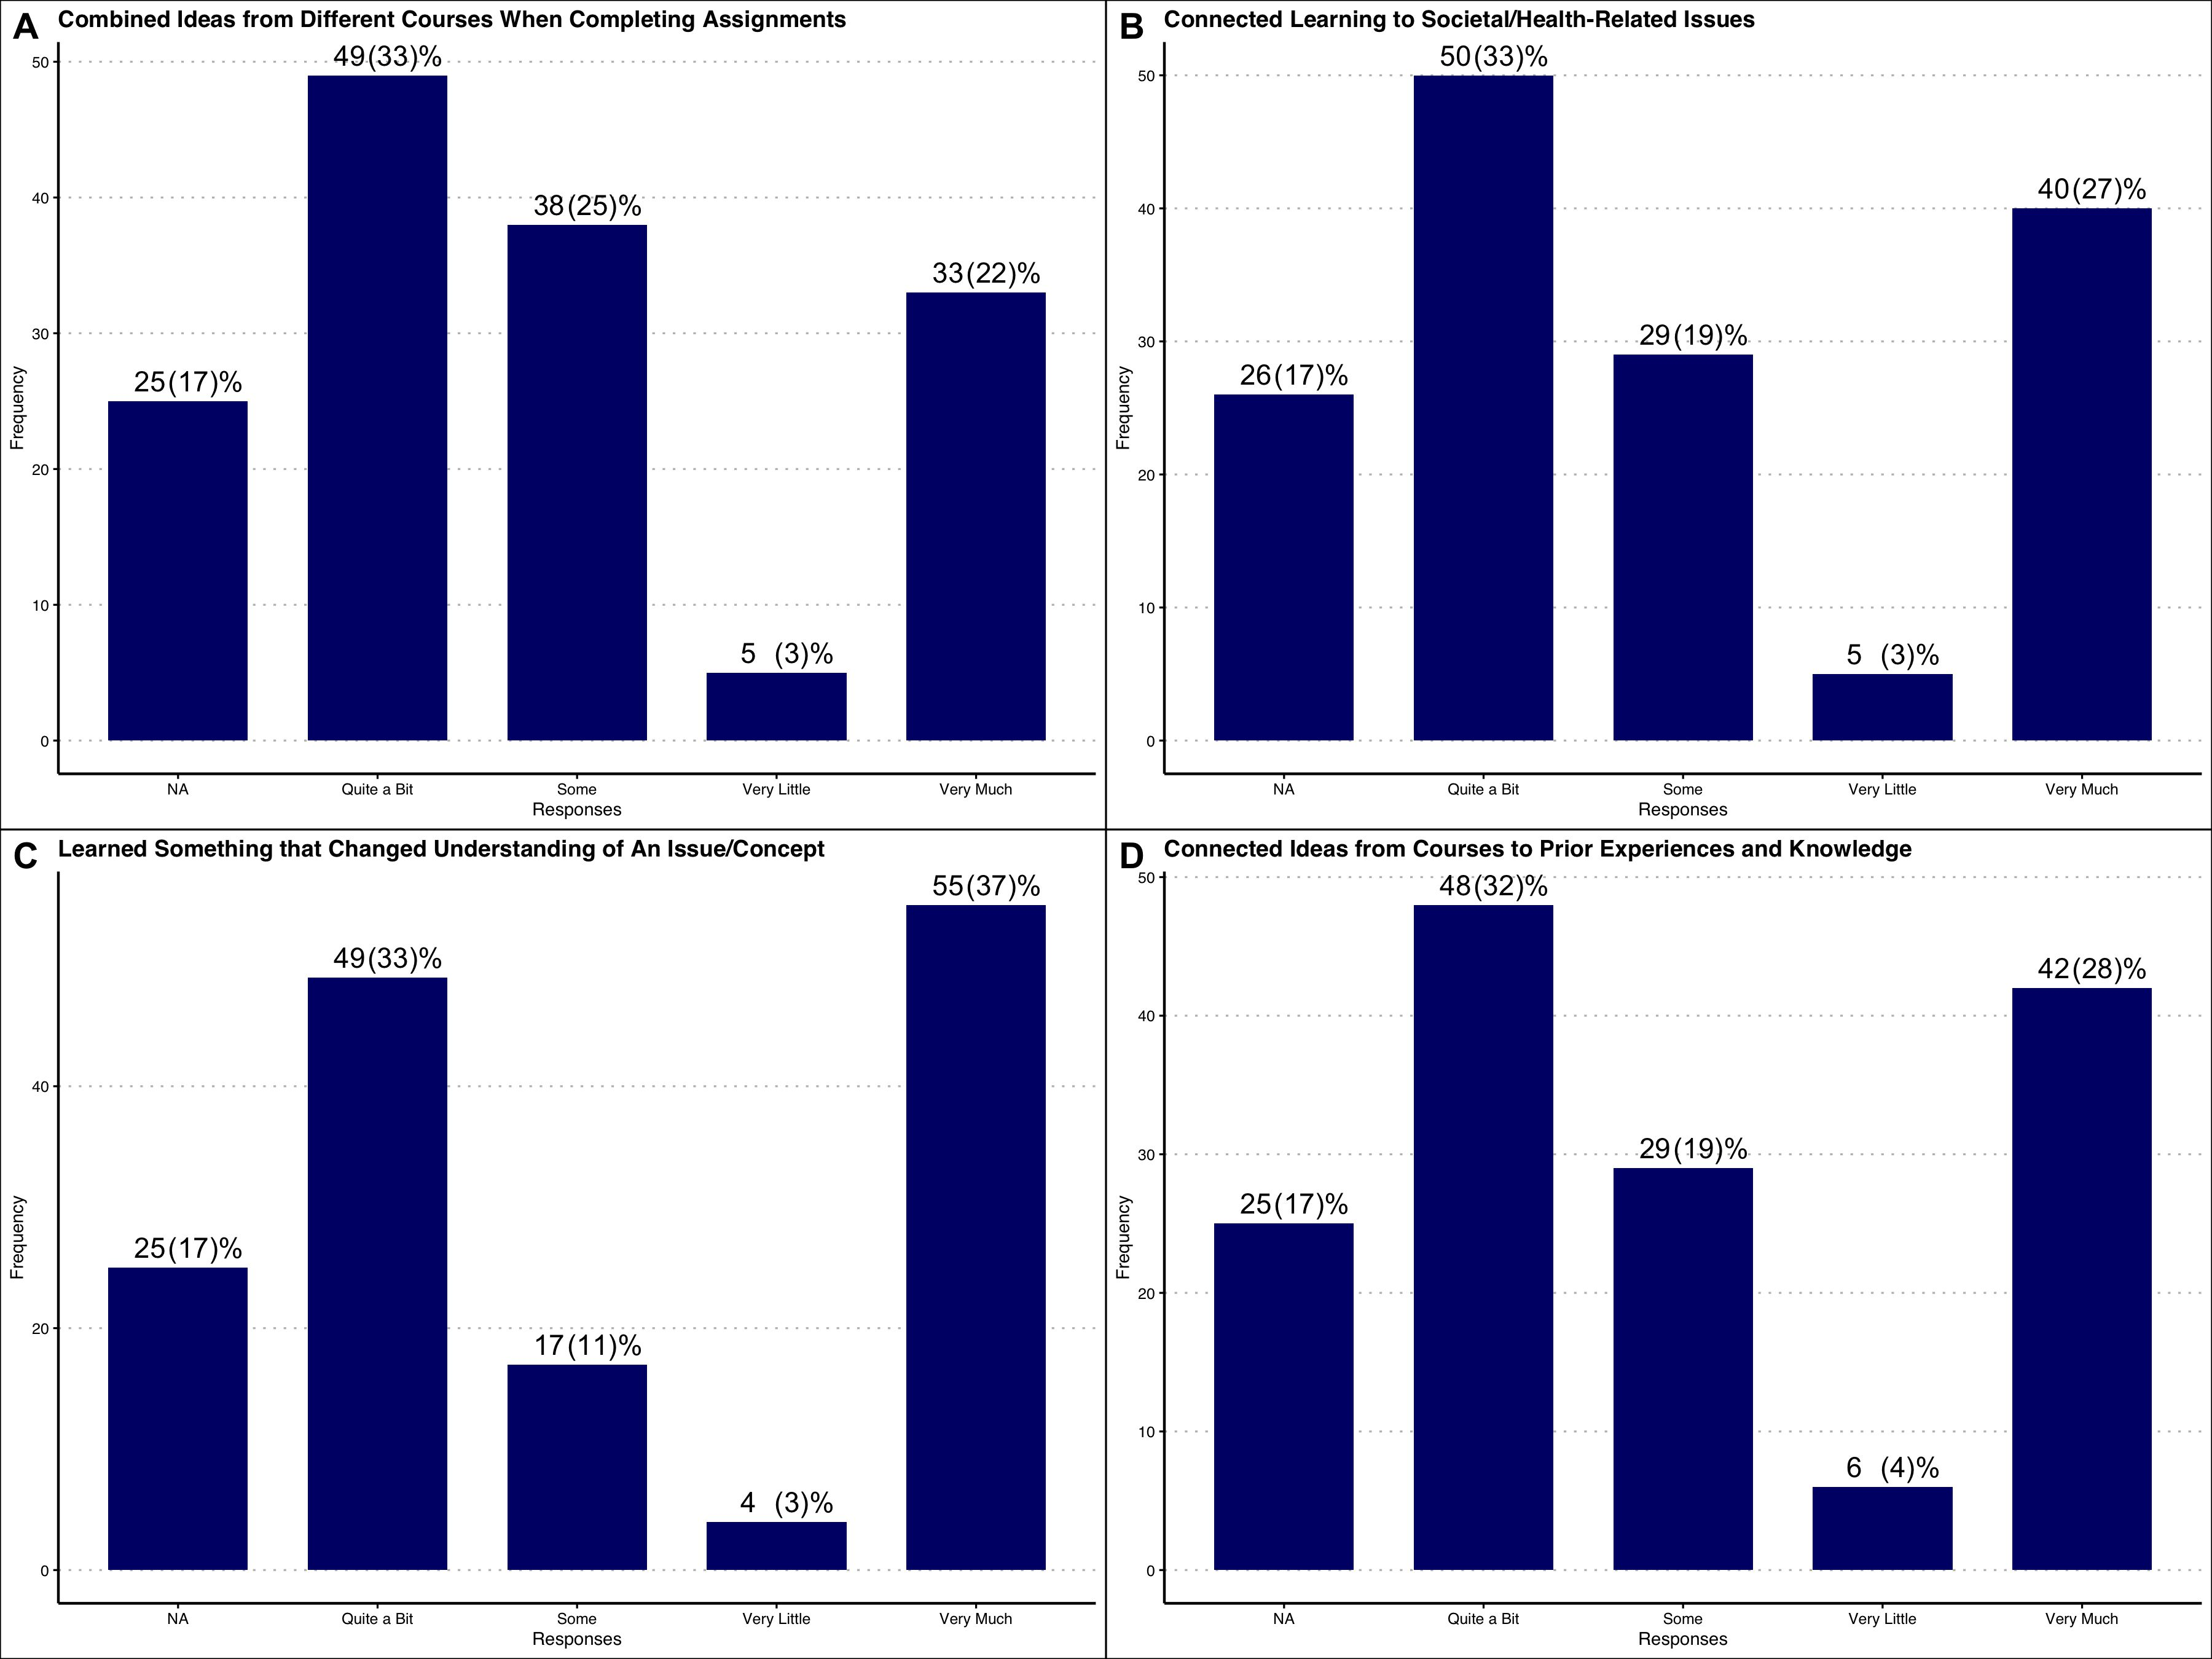
\includegraphics[width=10cm, height=6cm]{figures/how_does_gbl_help_in_science.jpg}
		\end{center}
		
	\end{frame}

	\begin{frame}{If BIO1A03 added a game-based learning component, how much would this improve your motivation to do the following? }
		
		\begin{center}
			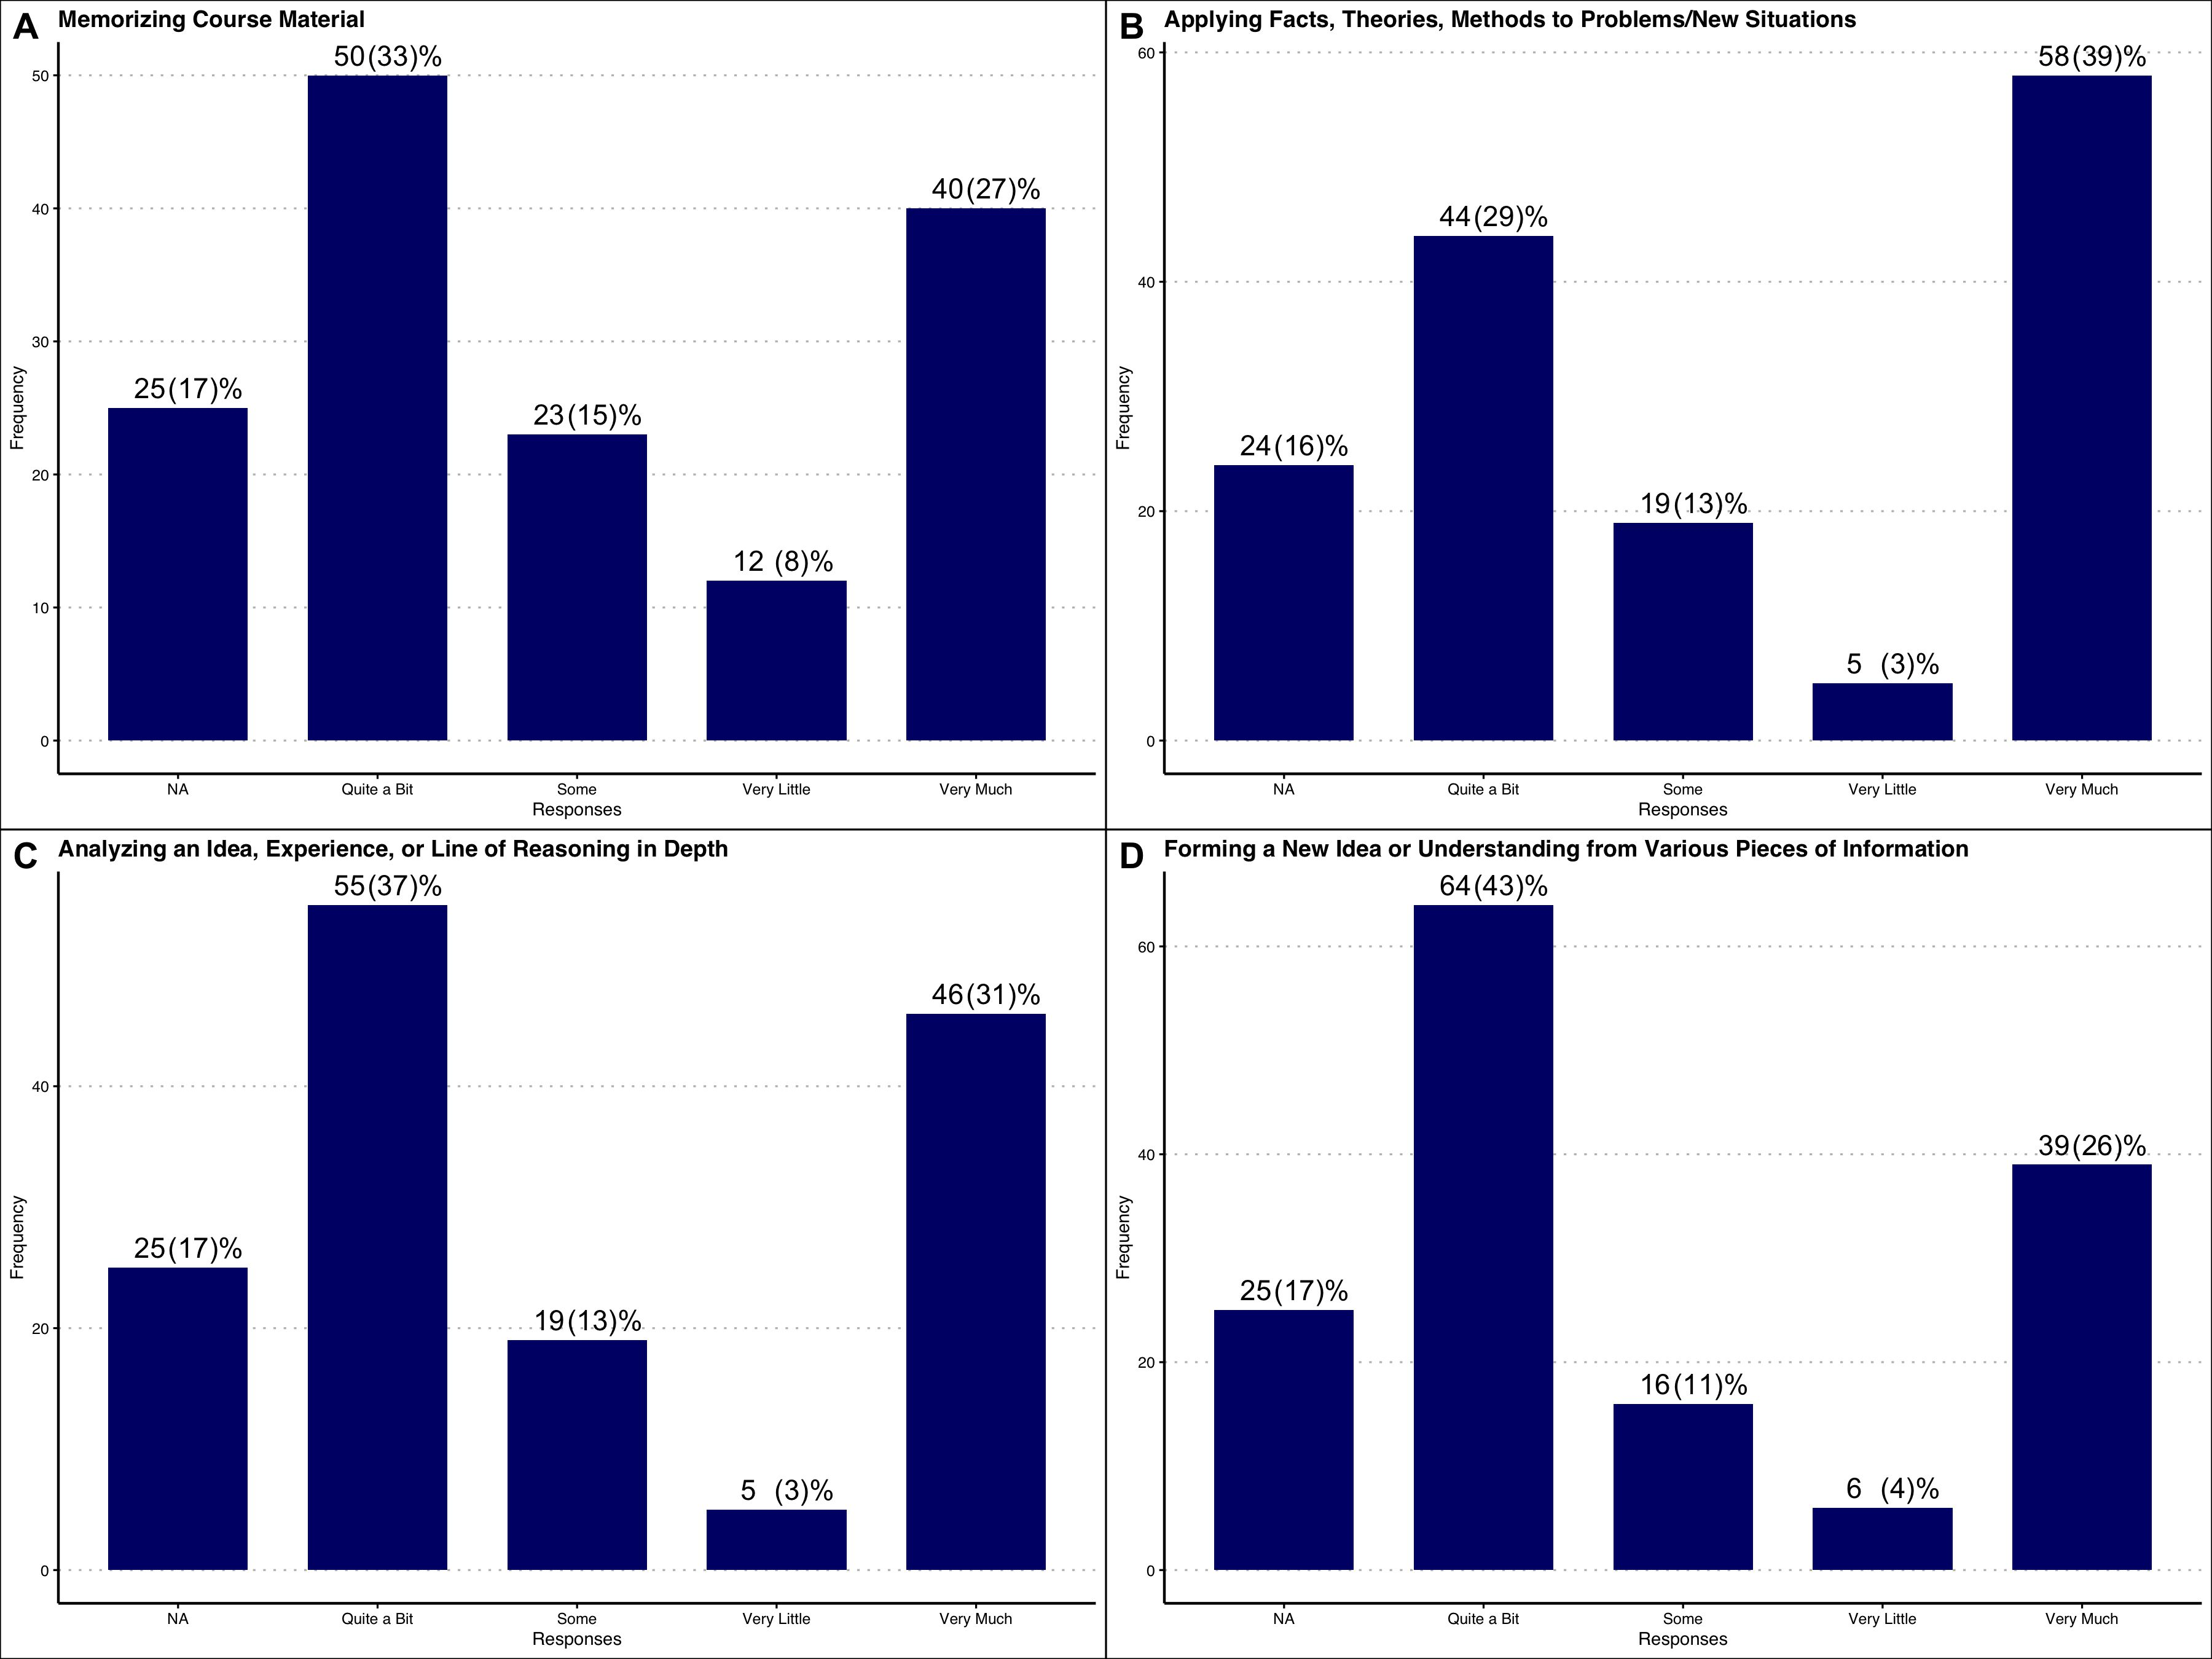
\includegraphics[width=10cm, height=6cm]{figures/ifbio1a03_added_gblcomponent.jpg}
		\end{center}
		
	\end{frame}

	\begin{frame}{How likely is it that you would play the video game Cells at War on your own time, outside of class to further consolidate material taught during this class? }
		
		\begin{center}
			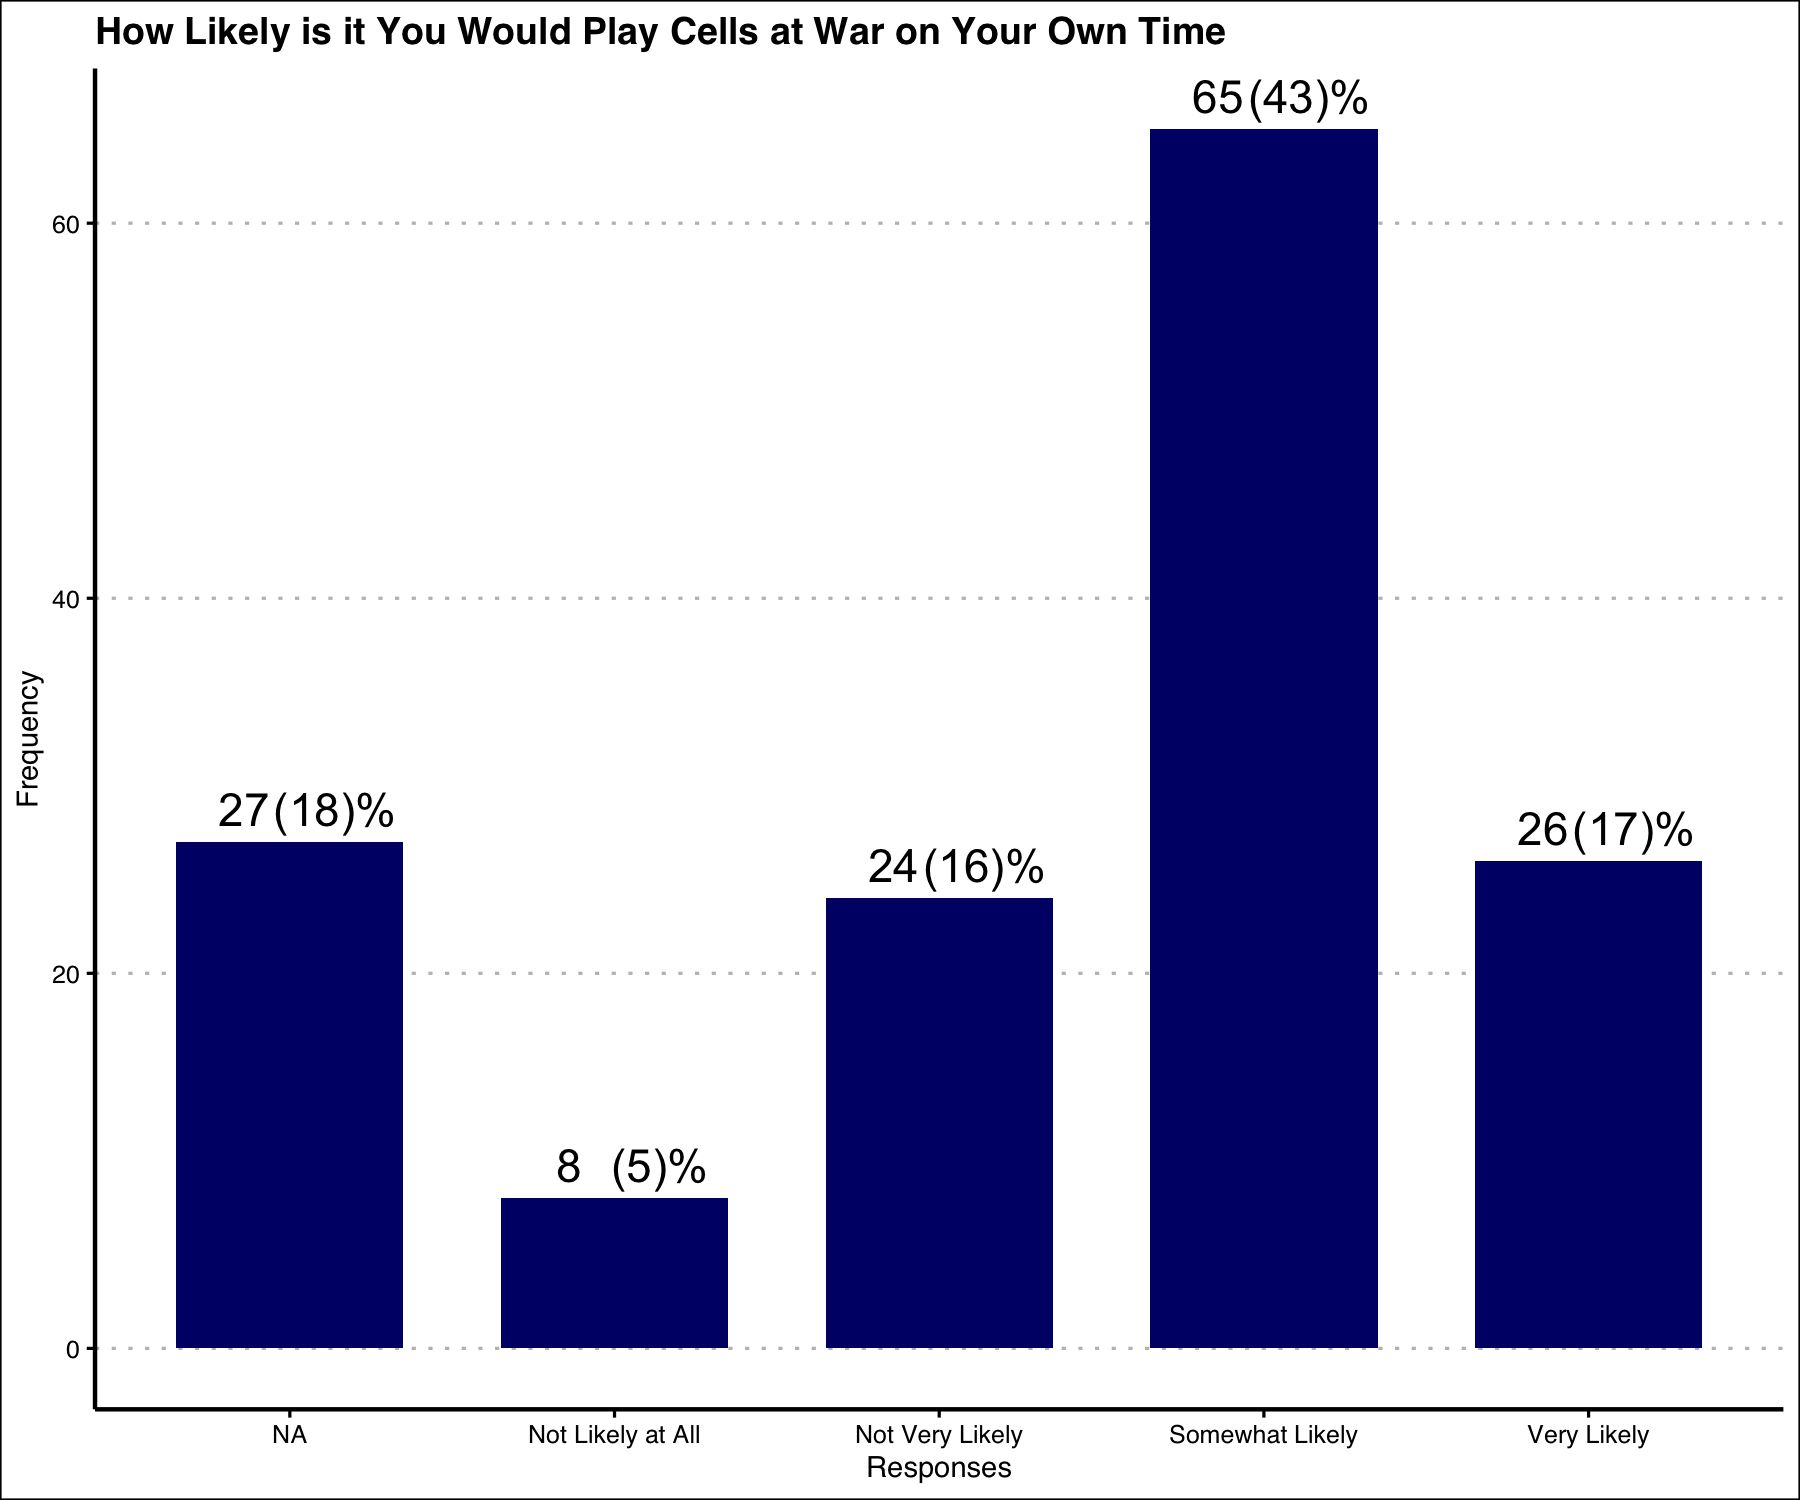
\includegraphics[width=9cm, height=6cm]{figures/how_likely_you_would_play_cellsatwar.jpg}
		\end{center}
		
	\end{frame}

	\begin{frame}{How prepared would you feel if you were given a quiz on Pompe Disease based on the Cells at War game, compared to studying off traditional lecture slides (with accompanying readings)? }
		
		\begin{center}
			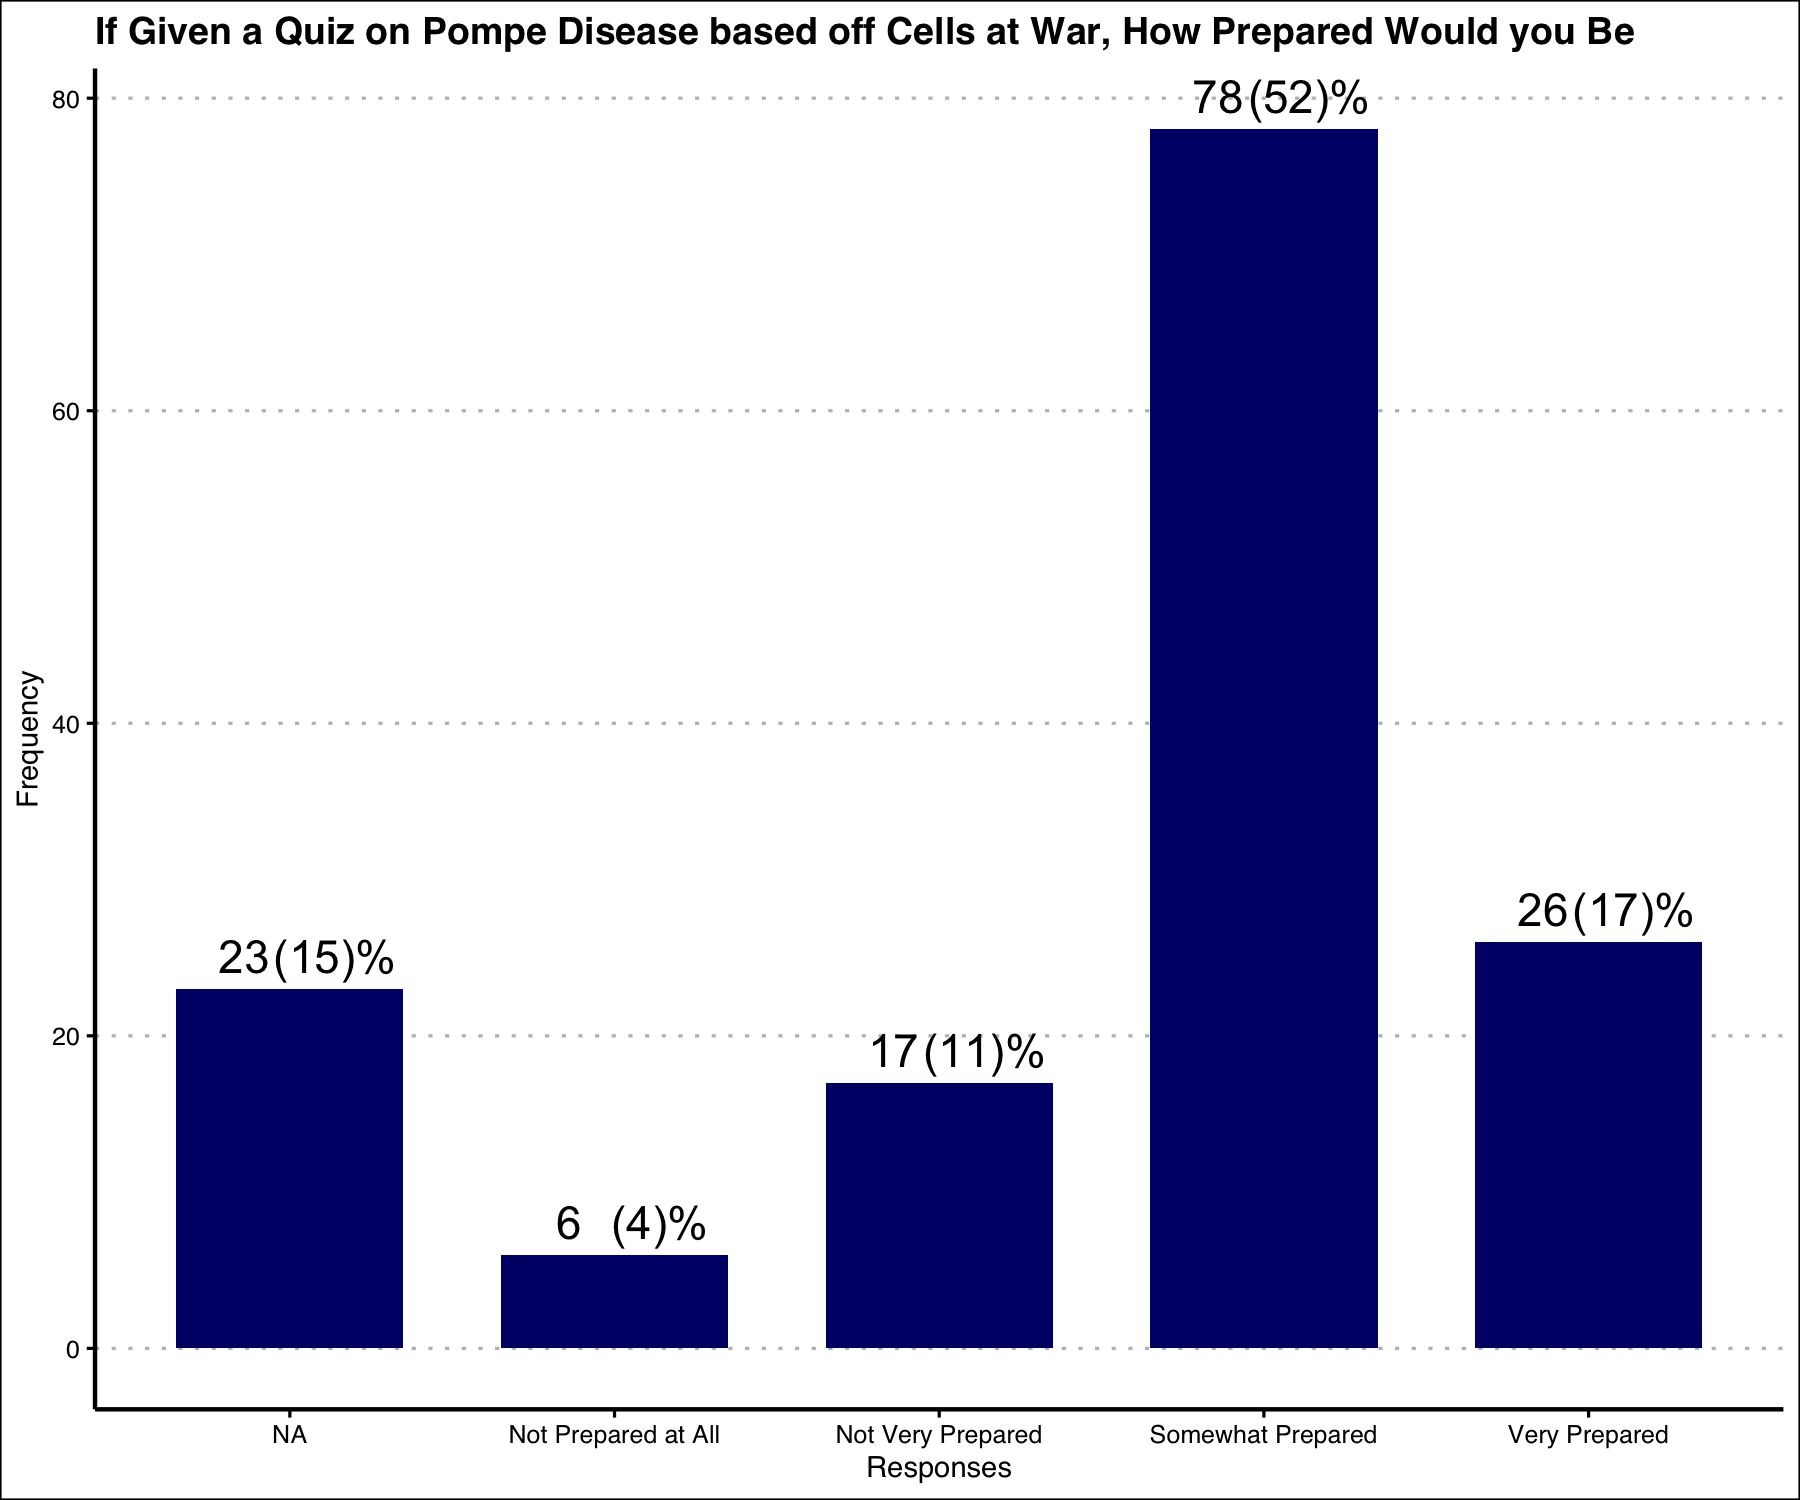
\includegraphics[width=9cm, height=6cm]{figures/how_prepared_if_tested_on_pompe_based_off_cellsatwar.jpg}
		\end{center}
		
	\end{frame}
	
\end{document}
